
\chapter{Inverse Laplace Transform}

%%%%%%%%%%%%%%%%%%%%%%%%%%%%%%%%%%%%%%%%%%%%%%%%%%%%%%%
\section{Definition}
The Laplace transform $F(p)$ of a function $f(t)$ is
\begin{equation}
  F(p) = \int_0^{\infty} f(t)\, e^{-pt} dt.
\end{equation}
The inverse Laplace transform $f(t)$ of a function $F(p)$ is
\begin{equation}
	f(t) = L_p^{-1} [ F(p) ] 
       = \frac{1}{2\pi i}   
           \int_{c-i\infty}^{c+i\infty} e^{p t} F(p)\, dp
\end{equation}

It is easy to see that
\begin{align*}
	F(a p+b) 
	&= \int_0^{\infty} f(t) e^{-(a p+b)t} dt  \\
	&= \int_0^{\infty} \frac{1}{a} f\left(\tau\right) e^{-b\tau /a} 
	     e^{-p\tau} d\tau  \qquad (\tau=a t),
\end{align*}
thus
\begin{equation} \label{E:ilt_lin}
	L_p^{-1} [ F(a p + b) ] = \frac{1}{a} f(\frac{t}{a}) e^{-b t/a}.
\end{equation}

It is useful to carry out the calculation a little further for a small circle
contour such as $EFG$ in Fig. \ref{F:cont1} as it reappears frequently. Let
$C_{\rho}$ be an arc with $p=\rho e^{i\theta}$ and we have
\[
  \int_{C_{\rho}}  
    = \frac{1}{2\pi i} \lim_{\rho\to 0} 
      \int e^{\rho e^{i\theta} t} F(\rho e^{i\theta})
        \rho e^{i\theta} i d\theta
    = \frac{\rho}{2\pi} \lim_{\rho\to 0} 
      \int_{C_{\rho}} e^{\rho t (\cos\theta+i\sin\theta)} F(\rho e^{i\theta})
         e^{i\theta} d\theta,
\]
and we have the inequality
\begin{equation}
  \lim_{\rho\to 0} \left| \int_{C_{\rho}} \right| 
    \le \lim_{\rho\to 0} \frac{\rho}{2\pi} 
      \int e^{\rho t \cos\theta} \left| F(\rho e^{i\theta}) \right| d\theta
    \le \lim_{\rho\to 0} \frac{\rho}{2\pi} e^{\rho t} 
        \int \left| F(\rho e^{i\theta}) \right| d\theta.
\end{equation}
One proposition of this is that if 
$\lim_{\rho\to 0} \rho |F(\rho e^{i\theta})|=0$ then we have 
$\lim_{\rho\to 0} \int_{C_{\rho}} =0$.


%%%%%%%%%%%%%%%%%%%%%%%%%%%%%%%%%%%%%%%%%%%%%%%%%%%%%%%
\section{ $ L_p^{-1} [ e^{-a\sqrt{p}} ], a>0 $ }
From definition, 
\[
	f(t)= L_p^{-1}\left[ e^{-a\sqrt{p}} \right]
	    = \frac{1}{2\pi i} 
			  \int_{c-i\infty}^{c+\infty} 
				e^{zt} e^{-a\sqrt{z}} dz.
\]
Since $z=0$ is a branch point, we use a contour around the branch cut from
$z=-\infty$ to $z=0$ (thus remaining in the principal branch) and have

%%%%%%%%%%%%%%%%%%%%%%%%%%%%%%%%%%%%
\begin{marginfigure} 
  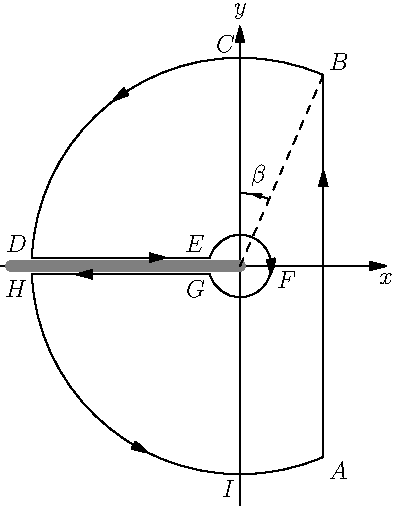
\includegraphics{graphics/contour.pdf}
\end{marginfigure}
%%%%%%%%%%%%%%%%%%%%%%%%%%%%%%%%%%%%

\[
  \oint = \int_{AB} + \int_{BCD} + \int_{DE} + \int_{EFG} + \int_{GH}
          + \int_{HIA}.
\]

Since the contour does not include any poles, using the residue theorem on the
principal branch $\sqrt{z}$ we get $\oint =0$. Now on contour $BCD$, 
$z=R e^{i\theta}$, $\frac{\pi}{2}-\beta <\theta <\pi$; while on contour $HIA$, 
$z=R e^{i\theta}$, $-\pi <\theta < -\frac{\pi}{2}+\beta$. Now on $BCD$ and
$HIA$, we have
\[
	\lim_{R\to \infty} \max_z |e^{-a\sqrt{z}}|
	= \lim_{R\to \infty} \max_{\theta} | e^{-a\sqrt{R} \cos\frac{\theta}{2}} |
	= \lim_{R\to \infty} e^{-a\sqrt{R}}
	= 0,
\]
thus by Jordan's Lemma (Corollary \ref{C:jordan}) we have
\[
  \int_{BCD} + \int_{HIA} = 0.
\]
And on the small circle contour $EFG$ we have
\[
	\int_{EFG} 
	= \frac{1}{2\pi i} 
	  \lim_{\epsilon\to 0} \int_{\pi}^{-\pi} e^{t\epsilon e^{i\theta}}
	    e^{-a\sqrt{\epsilon} e^{i\theta /2}} \epsilon e^{i\theta} i d\theta
	= 0.
\]

Along line $DE$, $z=x e^{i\pi}=-x$, where $x$ ranges from $\infty$ to $0$, and 
$\sqrt{z}=\sqrt{x} e^{i\pi /2}= i\sqrt{x}$, thus
\[
	\int_{DE} = \frac{1}{2\pi i} \int_{\infty}^0 e^{-tx} e^{-i a \sqrt{x}} (-dx).
\]
Similarly, along line $GH$, $z=x e^{-i\pi}=-x$, where $x$ ranges from $0$ to
$\infty$, and $\sqrt{z}=\sqrt{x} e^{-i\pi/2} = -i\sqrt{x}$, thus 
\[
	\int_{GH} = \frac{1}{2\pi i} \int^{\infty}_0 e^{-tx} e^{i a \sqrt{x}} (-dx).
\]
Hence
\[
	\int_{DE} + \int_{GH}
	= -\frac{1}{\pi} \int_0^{\infty} e^{-tx} \sin a\sqrt{x} dx
	= -\frac{2}{\pi t} 
	  \int_0^{\infty} e^{-u^2} \sin \left( \frac{a}{\sqrt{t}} u \right) u du,
\]
using Eq. \ref{E:int2_2}, we have
\[
	\int_{DE} + \int_{GH}
	= - \frac{a}{2\sqrt{\pi} t^{3/2}} e^{-a^2/4t}.
\]

Hence 
\begin{align*}
  \int_{AB} 
	&= \oint - \left( \int_{BCD} + \int_{HIA} \right)
     - \left( \int_{DE} + \int_{GH} \right) - \int_{EFG}  \\
  &= \frac{a}{2\sqrt{\pi} t^{3/2}} e^{-a^2/4t}, 
\end{align*}
i.e.
\footnote{cf. Borodin and Salemin, Handbook of Brownian Motions, 2ed, Appendix
3.2, Equation 2, p. 650}
\begin{equation} \label{E:ilt_1a}
	f(t)= L_p^{-1}\left[ e^{-a\sqrt{p}} \right]
      = \frac{a}{2\sqrt{\pi} t^{3/2}} e^{-a^2/4t}, \qquad a>0.
\end{equation}

%%%%%%%%%%%%%%%%%%%%%%%%%%%%%%%%%%%%%%%%%%%%%%%%%%%%%%%
\section{$ L_{\lambda}^{-1} 
\left( \frac{e^{-\alpha \sqrt{2\lambda}}}{\lambda(\sqrt{2\lambda}+\gamma)}
\right), \alpha > 0 $}
Let
\begin{align*}
  f(y) &= L_{\lambda}^{-1} 
          \left( 
            \frac{e^{-\alpha \sqrt{2\lambda}}}{\lambda(\sqrt{2\lambda}+\gamma)} 
          \right)    \\
       &= \frac{1}{2\pi i}   
           \int_{c-i\infty}^{c+i\infty} e^{\lambda y} 
           \frac{e^{-\alpha \sqrt{2\lambda}}}{\lambda(\sqrt{2\lambda}+\gamma)} 
           \, d\lambda.
\end{align*}
Since $\lambda=0$ is a branch point, we use the contour shown in Figure
\ref{F:cont1} and have
\[
  \oint = \int_{AB} + \int_{BCD} + \int_{DE} + \int_{EFG} + \int_{GH}
          + \int_{HIA}.
\]
Using the residue theorem (on the principal branch $\sqrt{\lambda}$) we get 
$\oint=0$. Using Jordan's Lemma we see
\[
  \int_{BCD} + \int_{HIA} = 0.
\]
%(remark that for contour HIA $F(\lambda)=
%\frac{e^{\alpha \sqrt{2\lambda}}}{\lambda(-\sqrt{2\lambda}+\gamma)}$).


%%%%%%%%%%%%%%%%%%%%%%%%%%%%%%%%%%%%
% \begin{figure} \label{F:cont1}
%   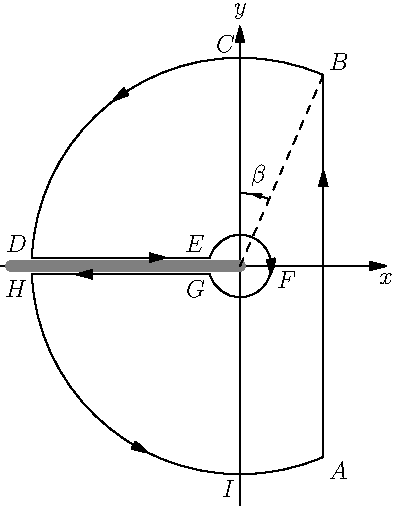
\includegraphics[width=3in]{graphics/contour.pdf}
% \end{figure}
\begin{marginfigure} \label{F:cont1}
  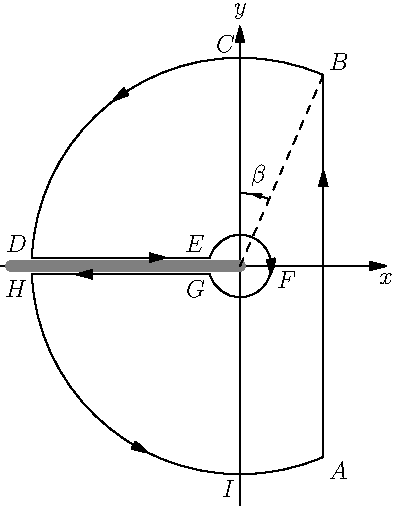
\includegraphics{graphics/contour.pdf}
	\caption{Contour.}
\end{marginfigure}
%%%%%%%%%%%%%%%%%%%%%%%%%%%%%%%%%%%%


It is easy to see that
\[
  \int_{EFG} = \frac{1}{2\pi i} \lim_{\epsilon \to 0} 
    \int_{\pi}^{-\pi} 
    \frac{ e^{ y \epsilon e^{i\theta} - \sqrt{2\epsilon} e^{i\theta/2} \alpha } }
         { \epsilon e^{i\theta} (\sqrt{2\epsilon} e^{i\theta/2} + \gamma) }
    \epsilon e^{i\theta} i d\theta
   = - \frac{1}{\gamma}.
\]
Along line $DE$, let $\lambda=x e^{i\pi}=-x$, 
and $\sqrt{2\lambda}=\sqrt{2x} e^{i\pi /2}=i \sqrt{2x}$, we get
\[
  \int_{DE} = \frac{1}{2\pi i} 
    \int_{\infty}^0 \frac{e^{-xy}}{x}\, 
      \frac{e^{-i\alpha\sqrt{2x}}}{\gamma+i\sqrt{2x}}\, dx.
\]
Similarly, along line $GH$, let $\lambda=x e^{-i\pi}=-x$, 
and $\sqrt{2\lambda}=\sqrt{2x} e^{-i\pi /2}=-i \sqrt{2x}$, we get
\[
  \int_{GH} = \frac{1}{2\pi i} 
    \int^{\infty}_0 \frac{e^{-xy}}{x}\, 
      \frac{e^{i\alpha\sqrt{2x}}}{\gamma-i\sqrt{2x}}\, dx.
\]
Hence
\begin{align*}
  \int_{DE} + \int_{GH} 
  &= \frac{1}{\pi} \int_0^{\infty} \frac{e^{-yx}}{x(\gamma^2+2x)}
       \left[
         \gamma \sin(\alpha \sqrt{2x}) + \sqrt{2x} \cos(\alpha \sqrt{2x})
       \right] \, dx  \\
  &= \frac{2\gamma}{\pi} \int_0^{\infty} 
       \frac{e^{-yu^2/2} \sin(\alpha u)}{u(u^2+\gamma^2)} \, du
     + \frac{2}{\pi} \int_0^{\infty} 
       \frac{e^{-yu^2/2} \cos(\alpha u)}{u^2+\gamma^2} \, du
\end{align*}
Using Equations \ref{E:int3} and \ref{E:int5}, we get
\[
  \int_{DE} + \int_{GH} 
  = \frac{1}{\gamma} e^{\alpha \gamma+\frac{1}{2}\gamma^2 y} 
      \erfc \left( \frac{\gamma \sqrt{y}}{\sqrt{2}}+ \frac{\alpha}{\sqrt{2y}} \right)
    + \frac{1}{\gamma} - \frac{1}{\gamma} \erfc \left( \frac{\alpha}{\sqrt{2y}}
\right).
\]
Hence 
\begin{align*}
  \int_{AB} &= \oint - \left( \int_{BCD} + \int_{HIA} \right)
               - \left( \int_{DE} + \int_{GH} \right) - \int_{EFG}  \\
            &= \frac{1}{\gamma} \erfc \left( \frac{\alpha}{\sqrt{2y}} \right)
               - \frac{1}{\gamma} e^{\alpha \gamma+\frac{1}{2}\gamma^2 y} 
                 \erfc 
                   \left( 
                     \frac{\gamma \sqrt{y}}{\sqrt{2}} + \frac{\alpha}{\sqrt{2y}} 
                   \right)
\end{align*}
This is exactly the inverse Laplace transform we are looking for
\begin{align} \label{E:ilt1}
  f(y) &= L_{\lambda}^{-1} 
          \left( 
            \frac{e^{-\alpha \sqrt{2\lambda}}}{\lambda(\sqrt{2\lambda}+\gamma)} 
          \right)   \notag \\  
       &= \frac{1}{\gamma} \erfc \left( \frac{\alpha}{\sqrt{2y}} \right)
          - \frac{1}{\gamma} e^{\alpha \gamma+\frac{1}{2}\gamma^2 y} 
            \erfc 
              \left( 
                \frac{\gamma \sqrt{y}}{\sqrt{2}}+ \frac{\alpha}{\sqrt{2y}} 
              \right)
\end{align}


%%%%%%%%%%%%%%%%%%%%%%%%%%%%%%%%%%%%%%%%%%%%%%%%%%%%%%%%%%%%%%%%%%%%%%%%%%%%%%%%
\section{$ L_{\lambda}^{-1}[ 
  \frac{1}{\sqrt{\lambda}} e^{-\alpha \sqrt{\lambda}} ] $ }
Use the same contour as in Figure \ref{F:cont1}, we get
\[
  \oint = \int_{AB} + \int_{BCD} + \int_{DE} + \int_{EFG} + \int_{GH}
          + \int_{HIA}.
\]
It is easy to see that $\oint=0$. Using Jordan's lemma, we have
\[
  \int_{BCD} + \int_{HIA} = 0.
\]
And
\[
  \int_{EFG} = \frac{1}{2\pi i} \lim_{\epsilon \to 0} 
    \int_{\pi}^{-\pi} e^{\epsilon e^{i\theta} y}
    \frac{1}{\sqrt{\epsilon} e^{i\theta/2}}
    e^{-\alpha \sqrt{\epsilon} e^{i\theta/2}}
    \epsilon e^{i\theta} \, i d\theta
  = 0. 
\]
Along line $DE$, let $\lambda=x e^{i\pi}=-x$, and 
$\sqrt{\lambda}=\sqrt{x} e^{i\pi/2}=i\sqrt{x}$, we get
\[
  \int_{DE} = -\frac{1}{2\pi} \int_0^{\infty} \frac{e^{-xy}}{\sqrt{x}}
              e^{-i\alpha x} \, dx.
\]
Similarly, along line $GH$, let $\lambda=x e^{-i\pi}=-x$, and 
$\sqrt{\lambda}=\sqrt{x} e^{-i\pi/2}=-i\sqrt{x}$, we get
\[
  \int_{GH} = -\frac{1}{2\pi} \int_0^{\infty} \frac{e^{-xy}}{\sqrt{x}}
              e^{i\alpha x} \, dx.
\]
Hence (using Equation \ref{E:int2} for the last step)
\begin{align*}
  \int_{DE} + \int_{GH} 
    &= -\frac{1}{2\pi} \int_0^{\infty} \frac{e^{-xy}}{\sqrt{x}}
       \left( e^{i\alpha x} + e^{-i\alpha x} \right) \, dx \\
    &= -\frac{1}{\pi} \int_0^{\infty} \frac{e^{-xy}}{\sqrt{x}}
         cos(\alpha \sqrt{x}) \, dx   \\
    &= - \frac{2}{\pi} \int_0^{\infty} e^{-yu^2} cos(\alpha u) \, du  \\
    &= - \frac{1}{\sqrt{\pi y}} e^{-\frac{\alpha^2}{4y}}
\end{align*}
Take all together and note that $f(y)=\int_{AB}$, we get
\begin{equation} \label{E:ilt2}
  f(y) = L_{\lambda}^{-1} 
         \left[ 
           \frac{1}{\sqrt{\lambda}} e^{-\alpha \sqrt{\lambda}}
         \right]
    = \frac{1}{\sqrt{\pi y}} e^{ -\frac{\alpha^2}{4y} } 
\end{equation}


%%%%%%%%%%%%%%%%%%%%%%%%%%%%%%%%%%%%%%%%%%%%%%%%%%%%%%
\section{ $ L_p^{-1} [ \frac{1}{\sqrt{p}(\sqrt{p}+b)} e^{-a\sqrt{p}} ], a\ge 0 $ }
From definition, 
\[
	f(t)= L_p^{-1}\left[ \frac{e^{-a\sqrt{p}}}{\sqrt{p}(\sqrt{p}+b)} \right]
	    = \frac{1}{2\pi i} 
			  \int_{c-i\infty}^{c+\infty} 
				e^{zt} \frac{e^{-a\sqrt{z}}}{\sqrt{z}(\sqrt{z}+b)} dz.
\]
Since $z=0$ is a branch point, we use a contour around the branch cut from
$z=-\infty$ to $z=0$ (thus remaining in the principal branch) and have

%%%%%%%%%%%%%%%%%%%%%%%%%%%%%%%%%%%%
\begin{marginfigure} 
  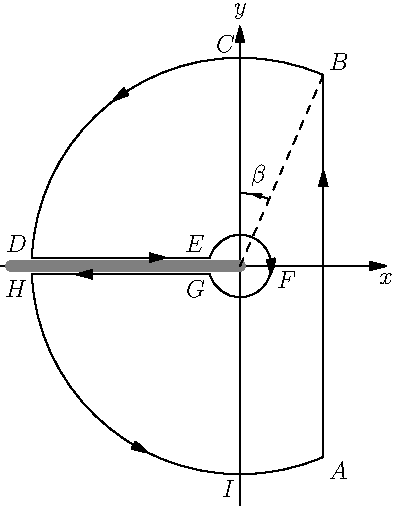
\includegraphics{graphics/contour.pdf}
\end{marginfigure}
%%%%%%%%%%%%%%%%%%%%%%%%%%%%%%%%%%%%

\[
  \oint = \int_{AB} + \int_{BCD} + \int_{DE} + \int_{EFG} + \int_{GH}
          + \int_{HIA}
\]

Since the contour does not include any poles, using the residue theorem on the
principal branch $\sqrt{z}$ we get $\oint =0$. 

Now on contour $BCD$, 
$z=R e^{i\theta}$, $\frac{\pi}{2}-\beta <\theta <\pi$; while on contour $HIA$, 
$z=R e^{i\theta}$, $-\pi <\theta < -\frac{\pi}{2}+\beta$. On $BCD$ and
$HIA$, we have
\[
  \lim_{R\to \infty} 
    \max_z \left| \frac{e^{-a\sqrt{z}}}{\sqrt{z}(\sqrt{z}+b)} \right|
  = \lim_{R\to \infty} \max_{\theta} 
      \left| 
        \frac{e^{-a\sqrt{R} e^{i\theta/2}}}
             { \sqrt{R} e^{i\theta/2} (\sqrt{R} e^{i\theta/2} + b) }
      \right|
  = 0,
\]
thus by Jordan's Lemma (Corollary \ref{C:jordan}) we have
\[
  \int_{BCD} + \int_{HIA} = 0.
\]
And on the small circle contour $EFG$ we have
\[
	\int_{EFG} 
	= \frac{1}{2\pi i} 
	  \lim_{\epsilon\to 0} \int_{\pi}^{-\pi} e^{t\epsilon e^{i\theta}}
	    \frac{e^{-a\sqrt{\epsilon} e^{i\theta/2}}}
             { \sqrt{\epsilon} e^{i\theta/2} (\sqrt{\epsilon} e^{i\theta/2} + b)}
        \epsilon e^{i\theta} i d\theta
	= 0.
\]

Along line $DE$, $z=x e^{i\pi}=-x$, where $x$ ranges from $\infty$ to $0$, and 
$\sqrt{z}=\sqrt{x} e^{i\pi /2}= i\sqrt{x}$, thus
\[
	\int_{DE} = \frac{1}{2\pi i} 
      \int_{\infty}^0 e^{-tx} 
        \frac{e^{-i a \sqrt{x}}}{i\sqrt{x}(i\sqrt{x}+b)} (-dx).
\]
Similarly, along line $GH$, $z=x e^{-i\pi}=-x$, where $x$ ranges from $0$ to
$\infty$, and $\sqrt{z}=\sqrt{x} e^{-i\pi/2} = -i\sqrt{x}$, thus 
\[
	\int_{GH} = \frac{1}{2\pi i}  
      \int^{\infty}_0 e^{-tx} 
        \frac{e^{i a \sqrt{x}}}{-i\sqrt{x}(-i\sqrt{x}+b)} (-dx).
\]
Hence
\begin{align*}
  \int_{DE} + \int_{GH}
	&= \frac{1}{\pi} 
      \int_0^{\infty} \frac{e^{-tx}}{\sqrt{x}(x+b^2)} 
        \left[ \sqrt{x}\sin(a\sqrt{x}) - b\cos(a\sqrt{x}) \right] dx \\
  &= \frac{2}{\pi} 
       \int_0^{\infty} \frac{e^{-t u^2} \sin(a u)}{u^2+b^2} \, u du
     -\frac{2b}{\pi} 
       \int_0^{\infty} \frac{e^{-t u^2} \cos(a u)}{u^2+b^2} \, du
\end{align*}
Using Equations \ref{E:int3} and \ref{E:int4}, we get
\[
  \int_{DE} + \int_{GH}
    = -e^{a b + b^2 t} \erfc\left( \frac{a}{2\sqrt{t}} + b \sqrt{t} \right)
\]

Hence 
\begin{align*}
  \int_{AB} 
	&= \oint - \left( \int_{BCD} + \int_{HIA} \right)
     - \left( \int_{DE} + \int_{GH} \right) - \int_{EFG}  \\
  &= e^{a b + b^2 t} \erfc\left( \frac{a}{2\sqrt{t}} + b \sqrt{t} \right)
\end{align*}
i.e.
\footnote{cf. Borodin and Salemin, Handbook of Brownian Motions, 2ed, Appendix
3.2, Equation 11, p. 650}
\begin{equation} \label{E:ilt_1a}
  f(t) = L_p^{-1} \left[ \frac{1}{\sqrt{p}(\sqrt{p}+b)} e^{-a\sqrt{p}} \right]
       = e^{a b + b^2 t} \erfc\left( \frac{a}{2\sqrt{t}} + b \sqrt{t} \right),
         \qquad a\ge 0 
\end{equation}



%%%%%%%%%%%%%%%%%%%%%%%%%%%%%%%%%%%%%%%%%%%%%%%%%%%%%%%%%%%%%%%%%%%%%%%%%%%%%%%%
\section{$ L_{\lambda}^{-1}[ 
  \frac{1}{\lambda} e^{-\alpha \sqrt{\lambda}} ] $ }
Let
\begin{align*}
  f(y) &= L_{\lambda}^{-1} 
          \left( 
            \frac{1}{\lambda} e^{-\alpha \sqrt{\lambda}} 
          \right)    \\
       &= \frac{1}{2\pi i}   
          \int_{c-i\infty}^{c+i\infty} e^{\lambda y} 
            \frac{1}{\lambda} e^{-\alpha \sqrt{\lambda}}  
            \, d\lambda.
\end{align*}
Since $\lambda=0$ is a branch point, we use the contour shown in Figure
\ref{F:cont1} and have
\[
  \oint = \int_{AB} + \int_{BCD} + \int_{DE} + \int_{EFG} + \int_{GH}
          + \int_{HIA}.
\]
Using the residue theorem (on the principal branch $\sqrt{\lambda}$) we get 
$\oint=0$. Using Jordan's Lemma we get
\[
  \int_{BCD} + \int_{HIA} = 0.
\]
It is easy to see that 
\[
  \int_{EFG} = \lim_{\epsilon \to 0} \frac{1}{2\pi i}
               \int_{\pi}^{-\pi} e^{y \epsilon e^{i\theta}}
               \frac{1}{\epsilon e^{i\theta}}
               e^{-\alpha \sqrt{\epsilon} e^{i\theta/2}}
               \epsilon e^{i\theta} i \, d\theta
             = -1.
\]
Along line $DE$, let $\lambda=x e^{i\pi}=-x$, and 
$\sqrt{\lambda}=\sqrt{x} e^{i\pi/2}=i\sqrt{x}$, we get
\[
  \int_{DE} = -\frac{1}{2\pi i} \int_0^{\infty} \frac{e^{-xy}}{x}
              e^{-i\alpha x} \, dx.
\]
Similarly, along line $GH$, let $\lambda=x e^{-i\pi}=-x$, and 
$\sqrt{\lambda}=\sqrt{x} e^{-i\pi/2}=-i\sqrt{x}$, we get
\[
  \int_{GH} = \frac{1}{2\pi i} \int_0^{\infty} \frac{e^{-xy}}{x}
              e^{i\alpha x} \, dx.
\]
Hence
\begin{align*}
  \int_{DE} + \int_{GH} 
    &= \frac{1}{\pi} 
      \int_0^{\infty} \frac{ e^{-xy} }{ x } \sin( \alpha \sqrt{x} ) \, dx \\
    &= \frac{2}{\pi} \int_0^{\infty} \frac{e^{-yu^2}}{u} \sin(\alpha u) \, du
\end{align*}
Using Equation \ref{E:int3} with $\gamma=0$, we get
\[
  \int_{DE} + \int_{GH} 
    =   \frac{1}{2} \erfc \left( -\frac{\alpha}{2\sqrt{y}} \right)
      - \frac{1}{2} \erfc \left( \frac{\alpha}{2\sqrt{y}}  \right).
\]

Hence 
\begin{align*}
  \int_{AB} 
	&= \oint - \left( \int_{BCD} + \int_{HIA} \right)
     - \left( \int_{DE} + \int_{GH} \right) - \int_{EFG}  \\
    & = 1 - \frac{1}{2} \erfc \left( -\frac{\alpha}{2\sqrt{y}} \right)
          + \frac{1}{2} \erfc \left( \frac{\alpha}{2\sqrt{y}}  \right) \\
    &= \erfc \left( \frac{\alpha}{2\sqrt{y}} \right) 
\end{align*}
i.e.
\footnote{cf. Borodin and Salemin, Handbook of Brownian Motions, 2ed, Appendix
3.2, Equation 6, p. 650}
\begin{equation}  \label{E:ilt3}
  f(y) = L_{\lambda}^{-1} 
         \left[ 
           \frac{1}{\lambda} e^{-\alpha \sqrt{\lambda}}
         \right]
       = \erfc \left( \frac{\alpha}{2\sqrt{y}} \right).
\end{equation}


%%%%%%%%%%%%%%%%%%%%%%%%%%%%%%%%%%%%%%%%%%%%%%%%%%%%%%%%%%%%%%%%%%%%%%%%
\section{$L_p^{-1}[ \erfc(\sqrt{ap}) ] $ }
Let 
\[
  F(p) = \erfc(\sqrt{ap}) 
       = \frac{2}{\sqrt{\pi}} \int_{\sqrt{ap}}^{\infty} e^{-x^2} dx,
\]
and we have
\[
  \frac{dF}{dp} = - \sqrt{\frac{a}{\pi}} \frac{e^{-ap}}{\sqrt{p}},
\]
and
\[
  \frac{d^2F}{dp^2} = \sqrt{\frac{a}{\pi}} \frac{e^{-ap}}{\sqrt{p}} 
                      \left( a + \frac{1}{2p} \right).
\]
Hence
\[
  p F"(p) + 2 F'(p) = a (-p F'(p) - F(p) ) + \frac{3}{2} F'(p) + a F(p),
\]
and the inverse Laplace transform of this equation is
\[
  (t^2-a t) f'(t) = (a-\frac{3}{2} t) f(t),
\]
where $f(t)$ is the inverse Laplace transform of function $F(p)$.
Solve this differential equation, we get
\[
  f(t) = \frac{A}{t \sqrt{t-a}} 1_{(a,\infty)}(t),
\]
here $A$ is the constant to be determined and we have used the fact that
$f(0)=\lim_{p \to \infty} p F(p) = 0$.

To determine the constant $A$, we take the Laplace transform of function
$\frac{A}{t \sqrt{t-a}} 1_{(a,\infty)}(t)$, this yields (using Equation
\ref{E:int6})
\[
  L\left[ f(t) = \frac{A}{t \sqrt{t-a}} 1_(a,\infty)(t) \right]
    = \frac{A}{\sqrt{a}} \int_1^{\infty} \frac{e^{-(ap)x}}{x \sqrt{x-1}} dx
    = \frac{A}{\sqrt{a}} \pi \erfc(\sqrt{ap}).
\]
Since this should be $\erfc(\sqrt{ap})$, we must have
$A=\sqrt{a}/\pi$, and 
\begin{equation}
  L_p^{-1}[ \erfc(\sqrt{ap}) ] = \frac{\sqrt{a}}{\pi t \sqrt{t-a}}
                                 1_{(a,\infty)}(t).
\end{equation}


%%%%%%%%%%%%%%%%%%%%%%%%%%%%%%%%%%%%%%%%%%%%%%%%%%%%%%%%%%%%%%%%%%%%%%%%
\section{$L_p^{-1}[ p^{-\nu} ], \nu>0 $ }
To invert function $p^{-\nu}$ for any $\nu>0$, first note that
for all positive integer $n$ we have
\[
  L_p^{-1} \left[ \frac{d^n}{dp^n} F(p) \right] = (-t)^n f(t).
\]
Thus for any $\nu>0$ let $n$ be the integral part of $\nu$ we have
\begin{align*} 
  L_p^{-1}[p^{-\nu}] 
    &= \left( \frac{-}{\nu-1} \right) 
        L_p^{-1} \left[\frac{d}{dp} p^{-(\nu-1)} \right] \notag \\
    &= \left( \frac{-}{\nu-1} \right) \left( \frac{-}{\nu-2} \right) 
        L_p^{-1} \left[\frac{d^2}{dp^2} p^{-(\nu-2)} \right] \notag \\
    &= \cdots  \notag \\
    &= \left( \frac{-}{\nu-1} \right) \left( \frac{-}{\nu-2} \right) 
       \cdots \left( \frac{-}{\nu-n} \right) 
        L_p^{-1} \left[\frac{d^n}{dp^n} p^{-(\nu-n)} \right], \notag \\
    &= \left( \frac{1}{\nu-1} \right) \left( \frac{1}{\nu-2} \right) 
       \cdots \left( \frac{1}{\nu-n} \right) 
       t^n L_p^{-1} \left[ p^{-(\nu-n)} \right], \notag \\
\end{align*}
that is
\begin{equation} \label{E:ilt_pow}
  L_p^{-1}[p^{-\nu}] 
    = \left( \frac{1}{\nu-1} \right) \left( \frac{1}{\nu-2} \right) 
      \cdots \left( \frac{1}{\nu-n} \right) 
      t^n L_p^{-1} \left[ p^{-(\nu-n)} \right].
\end{equation}
Hence we only need to invert the function with $0<\nu<1$.

To invert function $F(p)=p^{-\nu}$ with $0<\nu<1$ by contour integration we have
\[
  f(t) = L_p^{-1} \left[ p^{-\nu} \right]
       = \frac{1}{2\pi i}   
           \int_{c-i\infty}^{c+i\infty} e^{p t} p^{-\nu}\, dp
       = t^{\nu-1} 
           \frac{1}{2\pi i} \int_{c-i\infty}^{c+i\infty} e^{z} z^{-\nu}\, dz,
\]
For simplicity we use the notation
\[
   \int_{AB} = \frac{1}{2\pi i} \int_{AB} e^{z} z^{-\nu}\, dz,
\]
and similarly for integration over other contours.
Since $z=0$ is a branch point (in general) we use the following contour and 
from the residue theorem we have

%%%%%%%%%%%%%%%%%%%%%%%%%%%%%%%%%%%%
\begin{marginfigure} \label{F:cont2}
  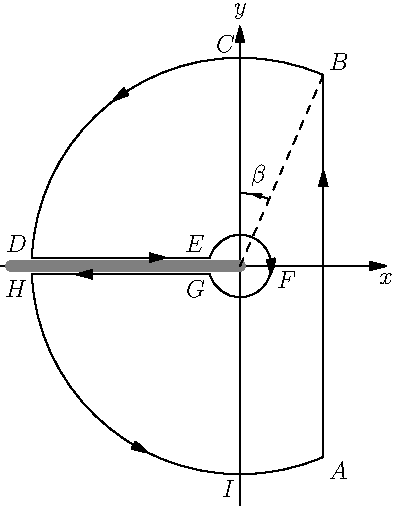
\includegraphics{graphics/contour.pdf}
\end{marginfigure}
%%%%%%%%%%%%%%%%%%%%%%%%%%%%%%%%%%%%

\[
  \oint = \int_{AB} + \int_{BCD} + \int_{DE} + \int_{EFG} + \int_{GH}
          + \int_{HIA} = 0.
\]

Note that from Jordan's lemma \ref{L:jordan} we have 
\[
  \int_{BCD}  + \int_{HIA} = 0.
\]
We also have $\int_{EFG}=0$ because
\[
  \lim_{\epsilon\to 0} |\int_{EFG} z^{-\nu} e^{z t} dz|
    \le \lim_{\epsilon\to 0} \int_{\pi}^{-\pi} \epsilon^{1-\nu} e^{\epsilon
        t\cos \theta} d\theta 
    = 0
\]
Along $DE$, $z=x e^{i\pi}$, thus
\[
  \frac{1}{2\pi i} \int_{DE} z^{-\nu} e^z dz
    = \frac{e^{-i\pi\nu}}{2\pi i} \int_0^{\infty} x^{-\nu} e^x dx,
\]
while along $GH$, $z=x e^{-i\pi}$, thus
\[
  \frac{1}{2\pi i} \int_{GH} z^{-\nu} e^z dz
    = - \frac{e^{i\pi\nu}}{2\pi i} \int_0^{\infty} x^{-\nu} e^x dx.
\]
Hence
\[
  \int_{DE} + \int_{GH}
    = - \frac{\sin(\nu\pi)}{\pi} \int_0^{\infty} x^{-\nu} e^x dx
    = - \frac{\sin(\nu\pi)}{\pi} \Gamma(1-\nu).
\]
and 
\[
  L_p^{-1} \left[ p^{-\nu} \right] = t^{\nu-1} \int_{AB}
    = \frac{\sin(\nu\pi)}{\pi} \Gamma(1-\nu).
\]
Using the Euler's reflection formula for gamma function (Proposition
\ref{P:gamma_pp}) we have
\begin{equation}
  L_p^{-1} \left[ p^{-\nu} \right] 
    = \frac{t^{\nu-1}}{\Gamma(\nu)}, \qquad 0<\nu<1.
\end{equation}

Using Eq. \ref{E:ilt_pow} and the simple property of gamma function
$\Gamma(z)=z\Gamma(z-1)$ we get
\begin{equation} \label{E:ilt4}
  L_p^{-1} \left[ p^{-\nu} \right] 
    = \frac{t^{\nu-1}}{\Gamma(\nu)}, \qquad \nu>0.
\end{equation}

%%%%%%%%%%%%%%%%%%%%%%%%%%%%%%%%%%%%%%%%%%%%%%%%%%%%%%%%%%%%%%%%%%%%%%%%
\section{$L_p^{-1}[ p^{-\mu} e^{a/p} ], \mu>0 $ }
Using Eq. \ref{E:ilt4} we get 
\begin{align*}
  L_p^{-1} \left[ p^{-\mu} e^{a/p} \right]
    &= L_p^{-1} 
       \left[ p^{-\mu} 
         \sum_{m=0}^{\infty} \left( \frac{a}{p} \right)^m \frac{1}{m!}
       \right]  \notag \\
    &= \sum_{m=0}^{\infty} \frac{a^m}{m!}
       L_p^{-1} \left[ \frac{1}{p^{m+\mu}} \right]  \notag \\
    &= \sum_{m=0}^{\infty} \frac{a^m}{m!}
       \frac{t^{\mu+m-1}}{\Gamma(\mu+m)}      \notag \\
    &= t^{\mu-1} \sum_{m=0}^{\infty} \frac{a^m t^m}{m!\Gamma(\mu+m)}. \notag\\
\end{align*}

From the definition of the modified Bessel function $I_{\nu}(z)$
\ref{D:bessel_mod}
we get
\begin{equation} \label{E:ilt5}
  L_p^{-1} \left[ p^{-\mu} e^{a/p} \right]
    = \left( \frac{t}{a} \right)^{\frac{\mu-1}{2}} I_{\mu-1}(2\sqrt{at})
      \qquad \mu>0.   
\end{equation}

An alternative method is to use differential equations.


%%%%%%%%%%%%%%%%%%%%%%%%%%%%%%%%%%%%%%%%%%%%%%%%%%%%%%%%%%%%%%%%%%%%%%%%
\section{$L_p^{-1}[ I_{\nu}(a\sqrt{2p}) K_{\nu}(b\sqrt{2p}) ]$ }
From the defintion we have
\[
  f(t)=L_p^{-1} \left[ I_{\nu}(a\sqrt{2p}) K_{\nu}(b\sqrt{2p}) \right]
   = \frac{1}{2\pi i}  \int_{c-i\infty}^{c+i\infty}
     e^{zt} I_{\nu}(a\sqrt{2z}) K_{\nu}(b\sqrt{2z})\, dz,
\]
Since $z=0$ is a branch point (in general) we use the following contour and 
from the residue theorem we have

\[
  \oint = \int_{AB} + \int_{BCD} + \int_{DE} + \int_{EFG} + \int_{GH}
          + \int_{HIA} = 0,
\]

%%%%%%%%%%%%%%%%%%%%%%%%%%%%%%%%%%%%
\begin{marginfigure} \label{F:cont3}
  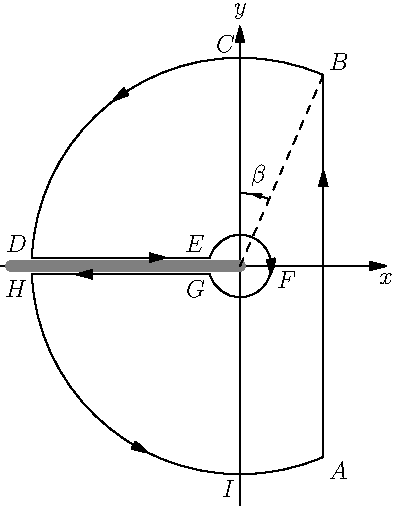
\includegraphics{graphics/contour.pdf}
\end{marginfigure}
%%%%%%%%%%%%%%%%%%%%%%%%%%%%%%%%%%%%

where for simplicity we use the notation
\[
   \int_{AB} = \frac{1}{2\pi i} 
      \int_{AB} e^{zt} I_{\nu}(a\sqrt{2z}) K_{\nu}(b\sqrt{2z})\, dz,
\]
and similarly for integration over other contours. 

First note that when $z\to\infty$ we have
\footnote{NIST Handbook of Mathematical Functions, 10.40.6 }
\[
  I_{\nu}(z) K_{\nu}(z) \sim \frac{1}{2z},
\]
thus from Jordan's lemma \ref{L:jordan} we have 
\[
  \int_{BCD}  + \int_{HIA} = 0,
\]

And note that when $z\to 0$ we have 
\[
  I_{\nu}(z) \sim \frac{1}{\Gamma(\nu+1)} \left( \frac{z}{2} \right)^{\nu},
\]
and
\[
  K_{\nu}(z) \sim \frac{\Gamma(|\nu|)}{2} \left( \frac{z}{2} \right)^{-|\nu|},
\]
hence when $\nu>-1$ we also have
\[
  \int_{EFG} = 0.
\]

Along $DE$, $z=x e^{i\pi}$, thus
\[
  \int_{DE} = \frac{1}{2\pi i} \int_0^{\infty} e^{-xt} 
    I_{\nu}(e^{i\pi/2} a\sqrt{2x}) K_{\nu}(e^{i\pi/2} b\sqrt{2x}) dx,
\]
while along $GH$, $z=x e^{-i\pi}$, thus
\[
  \int_{GH} = - \frac{1}{2\pi i} \int_0^{\infty} e^{-xt} 
    I_{\nu}(e^{-i\pi/2} a\sqrt{2x}) K_{\nu}(e^{-i\pi/2} b\sqrt{2x}) dx,
\]
Hence
\[
  \int_{DE} + \int_{GH} = - \frac{1}{2\pi i} 
    \int_0^{\infty} e^{-xt} 
    [ I_{\nu}(e^{-i\pi/2} a\sqrt{2x}) K_{\nu}(e^{-i\pi/2} b\sqrt{2x}) 
     - I_{\nu}(e^{i\pi/2} a\sqrt{2x}) K_{\nu}(e^{i\pi/2} b\sqrt{2x}) ] dx,
\]

From the definition of Bessel functions $J_{\nu}(z)$ and modified Bessel
functions $I_{\nu}(z)$ we get
\[
  I_{\nu}(e^{i\pi n/2} z) = e^{i\pi n\nu/2} J_{\nu}(z),
    \qquad n=\pm 1,\pm 3, \pm 5,\cdots
\]
Using this and the definition
$K_{\nu}(z)=\frac{\pi}{2\sin\pi\nu}(I_{-\nu}(z)-I_{\nu}(z))$ we thus get
\[
  I_{\nu}(e^{-i\pi/2} a\sqrt{2x}) K_{\nu}(e^{-i\pi/2} b\sqrt{2x}) 
    - I_{\nu}(e^{i\pi/2} a\sqrt{2x}) K_{\nu}(e^{i\pi/2} b\sqrt{2x}) 
  = i \pi \, J_{\nu}(a\sqrt{2x}) J_{\nu}(b\sqrt{2x}),
\]
and thus
\[
  f(t)= \int_{AB} = - \int_{DE} - \int_{GH} = \frac{1}{2} 
    \int_0^{\infty} e^{-xt} J_{\nu}(a\sqrt{2x}) J_{\nu}(b\sqrt{2x}) dx.
\]
Using Weber's second exponential integral
\footnote{Watson, A Treatise on the Theory of Bessel Functions, 13.31(1), p395}
\[
  \int_0^{\infty} e^{-p^2 t^2} J_{\nu}(at) J_{\nu}(bt)tdt
    = \frac{1}{2p^2} \exp\left( -\frac{a^2+b^2}{4p^2} \right)
      I_{\nu}\left( \frac{ab}{2p^2} \right)
      \qquad Re(\nu)>-1, |\arg p|<\pi/4
\]
we thus get
\begin{equation} \label{E:ilt6}
  L_p^{-1} \left[ I_{\nu}(a\sqrt{2p}) K_{\nu}(b\sqrt{2p}) \right]
    = \frac{1}{2t} \exp\left( -\frac{a^2+b^2}{2t} \right)
      I_{\nu} \left( \frac{ab}{t} \right) \qquad \nu>-1.
\end{equation}

%%%%%%%%%%%%%%%%%%%%%%%%%%%%%%%%%%%%%%%%%%%%%%%%%%%%%%%%%%%%%%%%%%%%%%%%%%
\section{$L_p^{-1}[ \frac{\sinh (\sqrt{p} a)}{\sinh (\sqrt{p} b)} ], |a|<b$ }
From definition we have
\[
  f(t)= L_p^{-1}\left[ \frac{\sinh (\sqrt{p} a)}{\sinh (\sqrt{p} b)} \right]
	    = \frac{1}{2\pi i} 
			  \int_{c-i\infty}^{c+\infty} 
		      e^{zt} \frac{\sinh (\sqrt{z} a)}{\sinh (\sqrt{z} b)} dz.
\]
Note first that
\begin{align*}
  e^{zt} \frac{\sinh (\sqrt{z} a)}{\sinh (\sqrt{z} b)} 
	&= \frac{ ( a\sqrt{z} + \frac{1}{3!} (a\sqrt{z})^3 
	            + \frac{1}{5!} (a\sqrt{z}^5 + \cdots )
							(1 + tz + \frac{(tz)^2}{2!} + \cdots) }
          { ( b\sqrt{z} + \frac{1}{3!} (b\sqrt{z})^3 
					    + \frac{1}{5!} (b\sqrt{z})^5 + \cdots ) } \\
	&= \frac{ (a + \frac{1}{3!} a^3 z + \frac{1}{5!} a^5 z^2 + \cdots)
            (1 + tz + \frac{(tz)^2}{2!} + \cdots) }
						{ (b + \frac{1}{3!} b^3 z + \frac{1}{5!} b^5 z^2 + \cdots) }, 
\end{align*}
thus $z=0$ is neither a pole nor a branch point.

Other poles are $z_n=-\frac{n^2 \pi^2}{b^2},n=1,2,3,\cdots$. 
The residues at the poles are
\[
	Res\left[ \frac{e^{tz} \sinh (\sqrt{z} a)}{\sinh (\sqrt{z} b)}; z_n \right] 
	= \lim_{z\to z_n} 
	  \frac{e^{t z} \sinh (\sqrt{z} a)}
	       { \frac{ \partial }{ \partial z } \sinh (\sqrt{z} b) }
	=  \frac{e^{t z_n} \sinh (\sqrt{z_n} a)}
          { \frac{b}{2\sqrt{z_n}} \cosh (\sqrt{z_n} b) }.
\]
It actually does not matter whether we choose $\sqrt{z_n}=\frac{n\pi i}{b}$ 
or $\sqrt{z_n}=- \frac{n\pi i}{b}$, and we always have
\[
	Res\left[ \frac{e^{tz} \sinh (\sqrt{z} a)}{\sinh (\sqrt{z} b)}; z_n \right] 
	= (-)^{n+1} \left( \frac{2n\pi}{b^2} \right) e^{-\frac{n^2\pi^2}{b^2} t} 
	  \sin(\frac{n\pi a}{b}).
\]

We select a simple contour that encloses all the poles, and we have

%%%%%%%%%%%%%%%%%%%%%%%%%%%%%%%%%%%%
\begin{marginfigure} 
  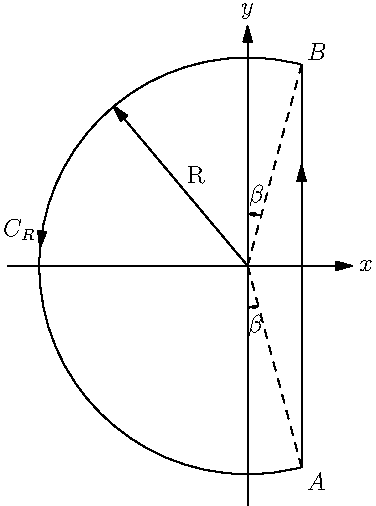
\includegraphics{graphics/contour_simple.pdf}
\end{marginfigure}
%%%%%%%%%%%%%%%%%%%%%%%%%%%%%%%%%%%%

\[
	\oint = \int_{AB} + \int_{C_R}.
\]
Now for $z=R e^{i\theta}$ on contour $C_R$,
$\frac{\pi}{2}-\beta<\theta<\frac{3}{2}\pi+\beta$. Since $|a|<b$, we have
\[
	\lim_{R\to\infty} \max_z \left| \frac{\sinh(\sqrt{z} a)}{\sinh (\sqrt{z} b)}
	\right|
	= \lim_{R\to\infty} \max_{\theta} e^{\sqrt{R} (|a|-b) |\cos\frac{\theta}{2}|}
	=0,
\]
thus by Jordan's Lemma (Corollary \ref{C:jordan}) we have $\int_{C_R}=0$.

Hence
\begin{align*}
	f(t)  
	&= \frac{1}{2\pi i}   
      \int_{c-i\infty}^{c+i\infty} e^{p t} F(p)\, dp  \\
	&= \frac{1}{2\pi i} \oint e^{z t} F(z)\, dz \\
	&= \sum_{n=1}^{\infty} 
	  Res\left[ \frac{e^{tz} \sinh (\sqrt{z} a)}{\sinh (\sqrt{z} b)}; z_n
		\right] \\
	&= \sum_{n=1}^{\infty} 
	  (-)^{n+1} \left( \frac{2n\pi}{b^2} \right) e^{-\frac{n^2\pi^2}{b^2} t} 
	  \sin(\frac{n\pi a}{b}).
\end{align*}
i.e.
\footnote{Doetsch, Introduction to the Theory and Application of the Laplace
Transformation, \#60, p.321; Spiegel, Schaum's Outline of Theory and Problems of
Laplace Transforms, Appendix B.124, p.252, note the missing of a negative sign.}
\begin{equation} \label{E:ilt_sinh_1A}
  f(t)
	= L_p^{-1}\left[ \frac{\sinh (\sqrt{p} a)}{\sinh (\sqrt{p} b)} \right]
	= \sum_{n=1}^{\infty} 
	  (-)^{n+1} \left( \frac{2n\pi}{b^2} \right) e^{-\frac{n^2\pi^2}{b^2} t} 
	  \sin(\frac{n\pi a}{b}).
\end{equation}

An alternative approach is the following. Observe that
\begin{align*}
	F(p) 
	&= \frac{\sinh (\sqrt{p} a)}{\sinh (\sqrt{p} b)}  
	 = \frac{e^{(a-b)\sqrt{p}} - e^{-(a+b)\sqrt{p}}}{1- e^{-2b\sqrt{p}}} \\
	&= (e^{(a-b)\sqrt{p}} - e^{-(a+b)\sqrt{p}}) 
	   \sum_{n=0}^{\infty} e^{-2nb\sqrt{p}} \\
  &= \sum_{n=0}^{\infty} 
		 \left( e^{-(-a+b+2nb)\sqrt{p}} - e^{-(a+b+2nb)\sqrt{p}} \right)
\end{align*}
Using Eq. \ref{E:ilt_1a} we get
\begin{align*}
	f(t) 
	&= L_p^{-1} [F(p)]  \\
  &= \sum_{n=0}^{\infty} 
	   \left( L_p^{-1}[ e^{-(-a+b+2nb)\sqrt{p}} ] 
	        - L_p^{-1}[ e^{-( a+b+2nb)\sqrt{p}} ] \right) \\
	&= \frac{1}{2\sqrt{\pi} t^{{3/2}} }
 		 \sum_{n=0}^{\infty} 
		 \left(
			 (-a+b+2nb) e^{-(-a+b+2nb)^2/4t} - (a+b+2nb) e^{-(a+b+2nb)^2/4t}
		 \right)  \\
  &= \frac{1}{2\sqrt{\pi} t^{{3/2}} }
 		 \sum_{n=-\infty}^{\infty}  (-a+b+2nb) e^{-(-a+b+2nb)^2/4t},
\end{align*}
i.e.,
\footnote{Doetsch, Introduction to the Theory and Application of the Laplace
Transformation, \#60, p.321 and p.200; cf. Borodin and Salemin, Handbook of 
Brownian Motions, 2ed, Appendix 2.11, p.641, defintion of $ss_y$.}
\begin{equation} \label{E:ilt_sinh_1B}
	L_p^{-1}\left[ \frac{\sinh (\sqrt{p} a)}{\sinh (\sqrt{p} b)} \right]
  = \frac{1}{2\sqrt{\pi} t^{{3/2}} }
 		\sum_{n=-\infty}^{\infty}  (-a+b+2nb) e^{-(-a+b+2nb)^2/4t}.
\end{equation}

We now verifty that Eq. \ref{E:ilt_sinh_1B} is equivalent to Eq.
\ref{E:ilt_sinh_1A}. 
Let
\[
  S_2 = \frac{1}{2\sqrt{\pi} t^{{3/2}} }
 		    \sum_{n=-\infty}^{\infty}  (-a+b+2nb) e^{-(-a+b+2nb)^2/4t},
\]
also let $y=\frac{a}{2b}$, we have
\[
	S_2 = \frac{b}{\sqrt{\pi} t^{3/2}}
	\sum_{n=-\infty}^{\infty}  (-y+\frac{1}{2}+n) e^{-(-y+\frac{1}{2}+n)^2 b^2/t},
\]
Now apply the Poisson summation formula, 
\footnote{Borwein and Borwein, Pi and the AGM, Theorem 2.2, p.37; Apostol,
Introduction to Mathematical Analysis, 2ed, pp.332-333.}
we get
\[
	S_2 
	= \sum_{n=-\infty}^{\infty} e^{2\pi i n y}
    \int_{-\infty}^{\infty} e^{-2\pi i n y}
		  \left( \frac{b}{\sqrt{\pi} t^{3/2}} \right)
      (-y+\frac{1}{2}+n) e^{-(-y+\frac{1}{2}+n)^2 b^2/t} \, dy.
\]
We first calculate the following integral
\begin{align*}
	I 
	&= \int_{-\infty}^{\infty} e^{-2\pi i n y}
      (-y+\frac{1}{2}+n) e^{-(-y+\frac{1}{2}+n)^2 b^2/t} \, dy \\
  &= \int_{-\infty}^{\infty} e^{-2\pi i n (x+\frac{1}{2} + n) }
			(-x) e^{-x^2 b^2/t} \, dx       \qquad (x=y-\frac{1}{2}-n) \\
	&= (-)^{n+1} \int_{-\infty}^{\infty} e^{-2\pi i n x} x e^{-x^2 b^2/t} \, dx \\
	&= (-)^n i \int_{-\infty}^{\infty} x \sin (2\pi n x) e^{-x^2 b^2/t} \, dx \\
	&= (-)^n i \frac{t}{b^2} \int_{-\infty}^{\infty} z 
			\sin \left( \frac{2\pi n \sqrt{t}}{b} z \right) e^{-z^2} \, dz,
			\qquad (z=\frac{x b}{\sqrt{t}}),
\end{align*}
using Eq. \ref{E:int2_2} we get
\[
	I = (-)^n i \frac{(\pi t)^{3/2}}{b^3} n e^{-\frac{n^2 \pi^2 t}{b^2}},
\]
hence
\begin{align*}
	S_2
	&= \sum_{n=-\infty}^{\infty} e^{2\pi i n y} \frac{b}{\sqrt{\pi}t^{3/2}}
	   \left( (-)^n i \frac{(\pi t)^{3/2}}{b^3} n e^{-\frac{n^2 \pi^2 t}{b^2}}
		 \right)  \\
  &= \sum_{n=-\infty}^{\infty} i e^{2\pi i n y} (-)^n \frac{n\pi}{b^2}
	       e^{-\frac{n^2 \pi^2 t}{b^2}}   \\
  &= \sum_{n=1}^{\infty} (-)^{n+1} \frac{2n\pi}{b^2} \sin(\frac{n\pi a}{b})
	     e^{-\frac{n^2 \pi^2 t}{b^2}}.
\end{align*}

For convenience we define the following theta function:
\footnote{Borodin and Salemin, Handbook of Brownian Motions, 2ed, Appendix 2.11, 
p.641, defintion of $ss_y$.}
\begin{align} \label{E:theta_ss}
	ss_t(a,b)
	&= L_p^{-1}\left[ \frac{\sinh (\sqrt{2p} a)}{\sinh (\sqrt{2p} b)} \right] 
	  \notag \\
	&= \frac{1}{\sqrt{2\pi} t^{{3/2}} }
 		 \sum_{n=-\infty}^{\infty}  (-a+b+2nb) e^{-(-a+b+2nb)^2/2t} \notag \\
  &= \sum_{n=1}^{\infty} (-)^{n+1} \frac{n\pi}{b^2} \sin(\frac{n\pi a}{b})
	     e^{-\frac{n^2 \pi^2 t}{2 b^2}},   
\end{align}
these two representations come from a straight-forward application of Eq. 
\ref{E:ilt_lin} on Eqs. \ref{E:ilt_sinh_1A} and \ref{E:ilt_sinh_1B}.

%%%%%%%%%%%%%%%%%%%%%%%%%%%%%%%%%%%%%%%%%%%%%%%%%%%%%%%%%%%%%%%%%%%%%%%%%%
\section{$L_p^{-1}[ \frac{\sinh (\sqrt{p} a)}{\sinh (\sqrt{p} b)} 
          \frac{e^{-c\sqrt{p}}}{\sqrt{p}} ], |a|<b, c>0$ }
Similar to the approach used in the previous section, we have
\[
	F[p] = \frac{\sinh (\sqrt{p} a)}{\sinh (\sqrt{p} b)} 
         \frac{e^{-c\sqrt{p}}}{\sqrt{p}} 
				 = \sum_{n=0}^{\infty} 
				 \left(
					 \frac{e^{-(-a+b+c+2nb)\sqrt{p}}}{\sqrt{p}}
					 -\frac{e^{-(a+b+c+2nb)\sqrt{p}}}{\sqrt{p}}
				 \right).
\]
Using Eq. \ref{E:ilt2} we get
\begin{align*}
	f(t)
	&= L_p^{-1}[F(p)]   \\
	&= \sum_{n=0}^{\infty} 
	   \left(
			  L_p^{-1} \left[ \frac{e^{-(-a+b+c+2nb)\sqrt{p}}}{\sqrt{p}} \right]
				-L_p^{-1} \left[ \frac{e^{-(a+b+c+2nb)\sqrt{p}}}{\sqrt{p}} \right]
		 \right) \\
	&= \sum_{n=0}^{\infty} 
	   \left(
			 \frac{ e^{-(-a+b+c+2nb)^2/4t} }{\sqrt{\pi t}}
			 - \frac{ e^{-(a+b+c+2nb)^2/4t} }{\sqrt{\pi t}}
		 \right), 
\end{align*}
i.e.
\begin{equation}
  L_p^{-1}\left[ \frac{\sinh (\sqrt{p} a)}{\sinh (\sqrt{p} b)} 
				         \frac{e^{-c\sqrt{z}}}{\sqrt{z}} \right]
	= \sum_{n=0}^{\infty} 
	   \left(
			 \frac{ e^{-(-a+b+c+2nb)^2/4t} }{\sqrt{\pi t}}
			 - \frac{ e^{-(a+b+c+2nb)^2/4t} }{\sqrt{\pi t}}
		 \right).
\end{equation}

Alternatively we can calculate the inverse Laplace transform using Bromwich 
integral:
\[
  f(t)= L_p^{-1}\left[ \frac{\sinh (\sqrt{p} a)}{\sinh (\sqrt{p} b)} 
				               \frac{e^{-c\sqrt{z}}}{\sqrt{z}} \right]
	    = \frac{1}{2\pi i} 
			  \int_{c-i\infty}^{c+\infty} 
		      e^{zt} \frac{\sinh (\sqrt{z} a)}{\sinh (\sqrt{z} b)} 
				  \frac{e^{-c\sqrt{z}}}{\sqrt{z}} 
				dz.
\]
Note that for function
\[
	F(z)= \frac{1}{2\pi i} e^{zt} \frac{\sinh (\sqrt{z} a)}{\sinh (\sqrt{z} b)} 
			  \frac{e^{-c\sqrt{z}}}{\sqrt{z}},
\]
$z=0$ is a branch point, and there are simple poles at
\[
	z_n=-\frac{n^2 \pi^2}{b^2}, n=1,2,3,\cdots,
\]
hence we select a contour around the branch cut from $z=-\infty$ to $z=0$ (thus
remain on the principal branch), and since all the poles are on the branch cut, 
we use semicircles around them. And we have

%%%%%%%%%%%%%%%%%%%%%%%%%%%%%%%%%%%%
\begin{marginfigure} 
  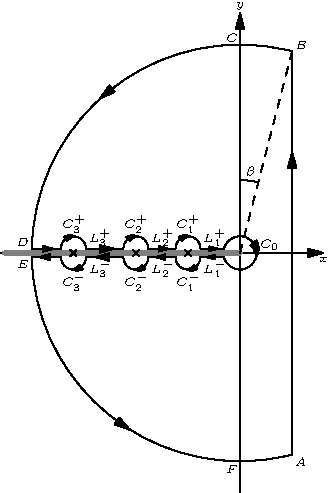
\includegraphics{graphics/contour_sinh.pdf}
	\caption{Contour with a branch cut from $z=-\infty$ to $z=0$ and semicircles
		around simple pole at $z_n=-\frac{n^2 \pi^2}{b^2}, n=1,2,3,\cdots$.}
\end{marginfigure}
%%%%%%%%%%%%%%%%%%%%%%%%%%%%%%%%%%%%

\[
	\oint F(z) dz 
	= \int_{AB} + \int_{BCD} + \int_{EFA} + \int_{C_0} 
	+ \sum_{n=1}^{\infty} 
	  \left( 
			\int_{C_n^+} + \int_{C_n^-} + \int_{L_n^+} + \int_{L_n^-} 
		\right)
 =0.
\]
Since the contour does not include any poles, using the residue theorem on the
principal branch $\sqrt{z}$ we get $\oint =0$. Now on contour $BCD$, 
$z=R e^{i\theta}$, $\frac{\pi}{2}-\beta <\theta <\pi$; while on contour $EFA$, 
$z=R e^{i\theta}$, $-\pi <\theta < -\frac{\pi}{2}+\beta$. Now on $BCD$ and
$EFA$, since $|a|<b$ and $c>0$, we have
\[
	\lim_{R\to\infty} \max_z 
	\left| 
	  \frac{\sinh(\sqrt{z} a)}{\sinh (\sqrt{z} b)} \frac{e^{-c\sqrt{z}}}{\sqrt{z}}
	\right|
	= \lim_{R\to\infty} \max_{\theta} 
	\frac{ e^{\sqrt{R} (|a|-b-c) \cos\frac{\theta}{2}} }
	     { \sqrt{R}\cos\frac{\theta}{2} }
	=0,
\]
thus by Jordan's Lemma (Corollary \ref{C:jordan}) we have 
\[
	\int_{BCD}=\int_{EFA}=0.
\]

And on the small circle $C_0$ we have
\[
	\int_{C_0} = \frac{1}{2\pi i} 
	  \lim_{\epsilon\to 0} \int_{\pi}^{-\pi} e^{t\epsilon e^{i\theta}}
		\frac{a\sqrt{\epsilon}e^{i\theta/2}}{b\sqrt{\epsilon}e^{i\theta/2}}
		\frac{e^{-c\sqrt{\epsilon}e^{i\theta/2}}}{\sqrt{\epsilon} e^{i\theta/2}}
		\epsilon e^{i\theta} i d\theta
	=0.
\]

On contour $C_n^+$, $z=z_n+\epsilon e^{i\theta}, 0<\theta<\pi$, thus
\[
	\sqrt{z}=\sqrt{z_n}+\frac{\epsilon e^{i\theta}}{2\sqrt{z_n}} + o(\epsilon^2),
\]
and
\begin{align*}
	\int_{C_n^+}
	&= \frac{1}{2\pi i} \lim_{\epsilon\to 0} \int_{\pi}^0 \epsilon e^{i\theta} i d\theta
	  \frac{e^{tz_n} \sinh(a\sqrt{z_n}) e^{-c\sqrt{z_n}}}
		{(-)^n \epsilon e^{i\theta} b/2}  \\
		&= \frac{(-)^{n+1}}{b} e^{tz_n} \sinh(a\sqrt{z_n}) e^{-c\sqrt{z_n}},
\end{align*}
while on contour $C_n^-$, $z=z_n e^{2\pi i}+\epsilon e^{i\theta}, \pi<\theta<2\pi$, 
thus
\[
	\sqrt{z}=-\sqrt{z_n}-\frac{\epsilon e^{i\theta}}{2\sqrt{z_n}} + o(\epsilon^2),
\]
and
\begin{align*}
	\int_{C_n^-}
	&= \frac{1}{2\pi i} \lim_{\epsilon\to 0} \int_{2\pi}^{\pi} \epsilon e^{i\theta} i d\theta
	  \frac{e^{tz_n} \sinh(-a\sqrt{z_n}) e^{c\sqrt{z_n}}}
		{(-)^{n} \epsilon e^{i\theta} b/2}  \\
		&= \frac{(-)^{n+1}}{b} e^{tz_n} \sinh(-a\sqrt{z_n}) e^{c\sqrt{z_n}} \\
		&= \frac{(-)^{n}}{b} e^{tz_n} \sinh(a\sqrt{z_n}) e^{c\sqrt{z_n}},
\end{align*}
hence
\begin{align*}
	\int_{C_n^+} + \int_{C_n^-}
	&= \frac{(-)^{n}}{b} e^{t z_n} \sinh(a\sqrt{z_n}) 
	   (e^{c\sqrt{z_n}} - e^{-c\sqrt{z_n}}) \\
		 &= (-)^n \frac{2}{b} e^{-\frac{n^2 \pi^2 t}{b^2}} \sin(\frac{n\pi a}{b}) 
        \sin(\frac{n\pi c}{b}).
\end{align*}

